\documentclass[11pt]{report}
\setlength{\headheight}{14pt}

\usepackage[a4paper, hmargin=2cm, vmargin=3cm]{geometry}
\usepackage[skip=11pt]{parskip}

\usepackage[T1]{fontenc}

\usepackage{hyperref}
\hypersetup{
    colorlinks=true,
    linkcolor=blue,
    filecolor=magenta,
    urlcolor=blue,
    bookmarksopen=true,
    pdftitle={Northport Manual}
}

\usepackage{enumitem}
\setitemize{noitemsep}

\usepackage{tikz}
\usetikzlibrary{positioning}
\usetikzlibrary{arrows.meta}
\usetikzlibrary{fit}
\usetikzlibrary{backgrounds}

\usepackage{titlesec}
\titleformat{\chapter}[hang]
    {\Huge\bfseries}
    {Chapter \thechapter\hspace{4pt}{|}\hspace{20pt}}
    {0pt}
    {\Huge\bfseries}

\usepackage{fancyhdr}
\pagestyle{fancy}
\fancyhf{}
\lhead{\leftmark}
\rfoot{Northport Manual}
\lfoot{Page \thepage}

\usepackage{listings}
\lstset{language=C++}
\lstset{basicstyle=\ttfamily}
\lstset{keywordstyle=\color{blue}}
\lstset{identifierstyle=\color{black}}
\lstset{commentstyle=\color{teal}}
\lstset{stringstyle=\color{red}}
\lstset{showstringspaces=false}
\lstset{backgroundcolor=\color{gray!10}}
\lstset{frame=l}
\lstset{emphstyle=\color{blue}}
\lstset{emph={void,PMM,VMM,Heap,uintptr_t,size_t,nullptr,Handle,NodeType,LogLevel}}
\lstset{emphstyle=[2]{\color{red!70!black!100}}}
\lstset{emph=[2]{ASSERT}}

\title{Northport Manual}
\author{Dean T, Northport Contributors}

\newcommand{\chapterpage}[1]{
    \pagestyle{empty}
    \chapter{#1}
    \newpage
    \pagestyle{fancy}
}

\newcommand{\drawlogo}{
    
\begin{tikzpicture}[baseline]
    \fill[black, draw=black] (2, 3) -- (5, 1) -- (5, 0) -- cycle;
    \fill[white, draw=black] (2, 3) -- (4, 0) -- (5, 0) -- cycle;
    \fill[black, draw=black] (8, 3) -- (6, 0) -- (5, 0) -- cycle;
    \fill[white, draw=black] (8, 3) -- (5, 1) -- (5, 0) -- cycle;
    \fill[black, draw=black] (8, -3) -- (5, -1) -- (5, 0) -- cycle;
    \fill[white, draw=black] (8, -3) -- (5, 1) -- (5, 0) -- cycle;
    \fill[black, draw=black] (2, -3) -- (5, 1) -- (5, 0) -- cycle;
    \fill[white, draw=black] (2, -3) -- (6, 0) -- (5, 0) -- cycle;

    \fill[black, draw=black] (0, 0) -- (4, 1) -- (5, 0) -- cycle;
    \fill[white, draw=black] (0, 0) -- (4, -1) -- (5, 0) -- cycle;
    \fill[black, draw=black] (5, 5) -- (6, 1) -- (5, 0) -- cycle;
    \fill[white, draw=black] (5, 5) -- (4, 1) -- (5, 0) -- cycle;
    \fill[black, draw=black] (10, 0) -- (6, -1) -- (5, 0) -- cycle;
    \fill[white, draw=black] (10, 0) -- (6, 1) -- (5, 0) -- cycle;
    \fill[black, draw=black] (5, -5) -- (4, -1) -- (5, 0) -- cycle;
    \fill[white, draw=black] (5, -5) -- (6, -1) -- (5, 0) -- cycle;
    \end{tikzpicture}
}

\begin{document}
\raggedright

\pagestyle{empty}
\pagenumbering{gobble}


\begin{titlepage}
    \begin{flushleft}
    \vspace{1cm}
    \Huge
    \textbf{Northport Manual}

    \rule{\textwidth}{2pt}
    \large
    Documentation for the kernel and supporting libraries.

    \vspace{4cm}
    \Large
    \center{\textit{N\hspace{-0.33em}P}}
    \center{\drawlogo}
    \vfill
    
    \begin{flushright}
    \small
    by
    \large
    \textbf{Dean T, Northport Contributors}
    
    \normalsize
    \today
    \end{flushright}

    \end{flushleft}
\end{titlepage}

\newpage
\newgeometry{vmargin=2cm, hmargin=4cm}
{
    \hypersetup{linkcolor=black}
    \tableofcontents
}
\restoregeometry
\newpage
\pagenumbering{arabic}
\pagestyle{fancy}

\chapterpage{Introduction}
\section{Preamble}
First of all, thanks for taking an interest in the project! If you're somehow reading this without a copy of the source code, there are copies hosted at the following sites:

\begin{itemize}
    \item Codeberg: \url{https://codeberg.org/r4/northport}
    \item GitHub: \url{https://github.com/deanoburrito/northport}
\end{itemize}

If you encounter any bugs or issues, feel free to open an issue on either of the repository mirrors listed above. If you just want to chat about the project the best way is on discord (\verb|r4#8873|).

\section{Contributors}
While git tracks contributors to the project, there has been a few rewrites over time, so for posterity a complete list of all contributors is maintained here. 

\begin{itemize}
    \item Dean T, \url{https://github.com/deanoburrito}
    \item Ivan G, \url{https://github.com/dreamos82}
\end{itemize}

\section{References \& Thanks}
I wanted to say a personal thanks to the following projects and resources, and the authors behind them, as they've helped me at various points throughout the development of northport. Any code from these projects has been licensed as appropriate, while some have been useful as a point of comparison, or helpful in understanding new concepts.

\begin{itemize}
    \item The Limine Bootloader: \url{https://github.com/limine-bootloader/limine}
    \item Nanoprintf: \url{https://github.com/charlesnicholson/nanoprintf}
    \item Qoi (Quite Ok Image) Format: \url{https://github.com/phoboslab/qoi}
    \item Frigg Utils Library: \url{https://github.com/managarm/frigg}
    \item Luna Hypervisor: \url{https://github.com/thomtl/Luna}
    \item SCAL-UX: \url{https://github.com/NetaScale/SCAL-UX}
    \item Ironclad: \url{https://www.nongnu.org/ironclad/}
    \item MentOS: \url{https://github.com/mentos-team/MentOS}
\end{itemize}

The builtin terminal font is \href{https://github.com/viler-int10h/vga-text-mode-fonts/blob/master/FONTS/NON-PC/APRIXENC.F14}{APRIXENC.F14} from \href{https://github.com/viler-int10h/vga-text-mode-fonts}{this collection} of x86 text mode fonts.

\section{License}

The source for this manual and all compiled copies fall under the same MIT license as the rest of the project. For completeness, a copy is embedded below:

\begin{verbatim}
MIT License

Copyright (c) Dean T.

Permission is hereby granted, free of charge, to any person obtaining a copy
of this software and associated documentation files (the "Software"), to deal
in the Software without restriction, including without limitation the rights
to use, copy, modify, merge, publish, distribute, sublicense, and/or sell
copies of the Software, and to permit persons to whom the Software is
furnished to do so, subject to the following conditions:

The above copyright notice and this permission notice shall be included in all
copies or substantial portions of the Software.

THE SOFTWARE IS PROVIDED "AS IS", WITHOUT WARRANTY OF ANY KIND, EXPRESS OR
IMPLIED, INCLUDING BUT NOT LIMITED TO THE WARRANTIES OF MERCHANTABILITY,
FITNESS FOR A PARTICULAR PURPOSE AND NONINFRINGEMENT. IN NO EVENT SHALL THE
AUTHORS OR COPYRIGHT HOLDERS BE LIABLE FOR ANY CLAIM, DAMAGES OR OTHER
LIABILITY, WHETHER IN AN ACTION OF CONTRACT, TORT OR OTHERWISE, ARISING FROM,
OUT OF OR IN CONNECTION WITH THE SOFTWARE OR THE USE OR OTHER DEALINGS IN THE
SOFTWARE.
\end{verbatim}

\section{Target Audience}
If you're reading this, you're probably the target audience. An intermediate level of C++ knowledge is expected, as is familiarity with working in a freestanding environment.

The purpose of this manual is document northport's design and implementation; not any of the hardware or protocols it may interact with. Descriptions of things external to the project will only be provided if necessary for another explanation.
Having said that, if you find something lacking or that could use clarification, feel free to let me know, or open a PR!

\section{Roadmap}
An up-to-date roadmap is kept in the source directory, at \verb|docs/roadmap.md|. This is where overall progress is tracked, broken down into individual features. Plans for future features are here too, but these will likely change over time.

A quick summary of the current features is also available in the project's readme, available in the root directory.

\section{Terminology}
Where possible, standard terminology is used to keep things accessible, but there are some less-standard terms and concepts used. For completeness they're described here:

\begin{itemize}
    \item \textbf{HHDM}: Higher Half Direct Map, a term borrowed from the Limine bootloader, this refers to an identity map of all physical memory that has been offset into the higher half. An identity map allows you to access physical memory at the same virtual address, and the HHDM works in a similar way but a fixed offset is added to the virtual address. This allows a full memory of physical memory to be accessible without impacting the lower half. The two fields used to manage this in the kernel (\verb|hhdmBase| and \verb|hhdmLength|) are determined once when the kernel is booted and are constant through the kernel's lifecycle. These values will only change when the kernel is booted, and are otherwise constant throughout it's lifetime. 
    \item \textbf{SUMAC}: A portmanteau of SUM (a riscv term) and SMAP (an x86 term), retconned to mean Supervisor/User Memory Access Control. SUMAC is enabled by default on systems where it's supported, and prevents the kernel from unintentionally accessing user memory. This feature is temporarily disabled when copying data in/out of the kernel address space during system calls, and otherwise is on at all times.
    \item \textbf{Extended Registers}: This term refers to any non-integer registers present in a processor. The kernel will always preserve integer registers on entry and exit, but extended registers are preserved lazily. Typically this is any floating point and vector registers that are present.
\end{itemize}

\section{Build System}
\label{Build System}
The entire project is built using GNU make, core utils and some platform-specific deployment tools. 

\subsection{Requirements}
\begin{itemize}
    \item GNU Make.
    \item Core utils (rm, mkdir, cp and friends).
    \item A cross compiler: GCC and clang are both supported.
    \item Xorriso.
    \item \href{https://github.com/limine-bootloader/limine}{The limine bootloader}. A binary release is fine, no need to build from source. See their instructions for how to download and install the latest release.
    \item A system root for the target platform. GCC cross compilers include this, clang does not and you will need to source your own.
\end{itemize}

The project is built as a series of smaller sub-projects, each living in their own directory. The root makefile combines a user config file (\verb|Config.mk|) and config file specific to the target platform (\verb|misc/cross/xyz/CrossCronfig.mk|) and populates some variables for compilation. These variables include compiler and linker flags, the toolchain binaries themselves, and how the final file should be presented (as an iso, or a plain kernel elf, depending on the target's requirements).

When a subproject is built, the root makefile recursively calls \verb|make| inside the project directly, and exports the previously created variables. Each subproject then builds itself, making use of the provided compiler flags and co.

The root makefile can be thought of as a glorified config mechanism, provoding settings to each subproject. The subproject's makefile then provides the scaffold of how to actually build the subproject, and the scaffold is filled in by the variables from the root makefile.

There are some additional files \verb|misc/BuildPrep.mk| and \verb|misc/RunDebug.mk| which provide useful functionality for interacting with the project, but are not directly related to building. \verb|RunDebug.mk| provides make targets for launching and debugging the kernel inside of qemu, and \verb|BuildPrep.mk| converts the user-facing options into compiler flags and pre-processor definitions.

\paragraph{Target Triplets}
The project currently uses the reduced versions of target triplets in the form of \verb|elf-$(ISA)|, where \verb|$(ISA)| is the target instruction set. As an example, this means any riscv64 platforms would use the target triplet \verb|elf-riscv64|, regardless of their ISA string (riscv64gcv for example). For x86\_64 the target triplet is \verb|elf-x86_64|.

In practice, target triplets are used to select toolchain binaries used for GCC, and given as the \verb|--target=| parameter for clang.

\paragraph{Libraries}
So far only a single library exists, but more are planned. Common make rules and targets are defined in a separate file (\verb|misc/LibCommon.mk|) which can then be included into a library's makefile. This is to save duplicating common build code across all libraries.

\paragraph{Kernel Syslib}
The \verb|np-syslib| library is actually built twice: once with the usual flags, and a second time with kernel-appropriate flags. The kernel version (\verb|knp-syslib|) is linked with the kernel, and has more restrictions placed on the code generation (for example, it only uses integer registers). Other programs and libraries are free to use the kernel version of np-syslib, and while there is no harm in doing so it is not recommended due to the extra restrictions placed on kernel code.

\subsection{Configuration}
Configuration is done in two places: at a global level in \verb|Config.mk|, and at a platform-specific level in \verb|misc/xyz/CrossConfig.mk|, where xyz is the target platform.

The global config is where you can set the cross-compiler paths, select the compiler you want to use and other common options like your target platform. The available options are documented in the config file itself.

Each supported platform has it's own \verb|CrossConfig.mk| file, where some platform specific compiler and linker flags can be set (like the codemodel). Other actions can be taken here as well, like changing the default build target. The available options are described below.

\begin{itemize}
    \item \verb|KERNEL_CXX_FLAGS|: This variable contains all the C++ compiler flags used for the kernel. Only platform-specific flags should be added here, for flags that affect all platforms add them in \verb|Config.mk|.
    \item \verb|KERNEL_LD_FLAGS|: For adding to the kernel linker flags, similar to the above option.
    \item \verb|ARCH_DEFAULT_TARGET|: Sets the makefile target to be used for \verb|make all|. Different platforms may require the kernel/system to be in different formats, UEFI systems accept a bootable iso for example. Some other systems may only support the bare kernel binary. Currently two builtin targets are provided: \verb|binaries| just compiles the kernel binary, and \verb|iso| which creates a UEFI iso with limine and the kernel.
    \item \verb|QEMU_BASE|: Base flags and the qemu binary to use.
    \item There are some other \verb|QEMU_*| flags that are added to the base flags depending on which make target is used (KVM/no KVM, UEFI/no UEFI).
\end{itemize}

\subsection{Make Targets}
The following make targets are available in the root makefile (i.e. from the project root directory). This is the intended interface into the build system.

While GNUmake is used for the build system, northport \textbf{does not} make use of dependency files (\verb|.d|) currently, so changes to \verb|.cpp| source files will trigger a rebuild of that file, changes to a \verb|.h| header file will not trigger rebuilds in affected source files. To test changes made to a header file, the recommended approach is to run \verb|make clean| followed by \verb|make| to perform a clean rebuild.

\begin{itemize}
    \item \verb|make|: Prints the help text, showing a summary of available make targets and notable files.
    \item \verb|make all|: Performs an incremental build of everything, and then performs a platform-specific packaging step. This might include burning a bootloader to an iso file, or leaving the kernel binary as is.
    \item \verb|make clean|: Completely removes all build files, resulting in the next build starting from scratch.
    \item \verb|make run|: Creates a platform-specific package, and launches it in qemu for the target architecture. By default this tries to use KVM.
    \item \verb|make run-kvmless|: Same as above, but explicitly disables use of KVM.
    \item \verb|make debug|: Similar to \verb|run|, but halts the virtual machine and starts the qemu gdb server with default arguments.
    \item \verb|make attach|: The other half of \verb|debug|, launches gdb with the kernel symbols loaded, and attempts to connect the qemu gdb server (default settings: tcp/1234).
    \item \verb|make docs|: Renders the documentation as a pdf.
    \item \verb|make docs-clean|: Removes temporary build files related to docs, useful after updating latex toolchain or a buggy build.
\end{itemize}

\subsection{Development Cycle}
For the initial setup you'll need to clone the repository, install any missing tools from the list above, and then adjust the global config (\verb|Config.mk|) to suit your environment. After opening a shell in the project root directory, and executing \verb|make run| the project should build and qemu should launch with the kernel. If this works then you're good to go.

General development is straightforward, \verb|make run| can be used to build the latest changes and test them. If you need to debug you can use \verb|make debug| in one terminal to launch qemu and \verb|make attach| in another to launch and attach gdb. As mentioned previously header files are not tracked as dependencies, so a clean build may be required when editing those.

Performing a clean build is also required when changing the target architecture, as the ISA the file was compiled for is not tracked. If a clean build is not performed you may encounter linker errors.

\section{Project Layout}
At the root level, the kernel and initdisk sources are available as separate directories, alongside \verb|libs/| which contains project directories for any support libraries.

The \verb|initdisk/| directory contains files used to build the initial ramdisk, which houses non-critical but nice-to-have files for the kernel. This subproject can contain all kinds of assets, not just source code.

The \verb|kernel/| source tree roughly shows the various kernel subsystems. For example the \verb|kernel/cpp/| directory contains code required to support some C++ language features, like the stack protector implementation, program sanitizers or stub functions required to be implemented by the C++ standard. The \verb|kernel/config/| directory contains code used for detecting the configuration of the current system, and so on.

The kernel also contains an \verb|kernel/arch/| directory, which is special. Only \textit{one} of the subdirectories is included when building the project. The name of the included subdirectory is derived from the target architecture of the compilation. As an example, if the kernel is being built for riscv64, only \verb|kernel/arch/riscv64| is included in the compilation process, not \verb|kernel/arch/x86_64| or any other architecture folder. This logic also applies to the include paths used for headers.

All subprojects that provide header files will make them available under an \verb|include/| directory inside the subproject's root directory.

Most projects will store build-artefacts under a \verb|build/| directory within their subproject folder. The \verb|build/| directory is purged on a clean build, and it's contents shouldn't be relied upon for anything other than potentially reducing compile times.

\subsection{Documentation}
As you might expect, the \verb|docs/| directory contains files related to documentation. The top level contains a handful of files like the project roadmap, and basic build instructions for those who don't want to (or cant) build the documentation.

The \verb|docs/manual/| directory contains the \LaTeX \hspace{0.25em}source for building this document, organised into relevant chapters.

Project imagery is also stashed in \verb|docs/images/|. This \textbf{does not} mean screenshots (which are stored external to the git repository) but rather banners and icons for use in the documentation.

\subsection{Miscellanious}
The \verb|misc/| directory contains a few things. Binary assets for the built-in terminal are stored here (\verb|misc/TerminalFont|, and optionally \verb|misc/TerminalBg.qoi|). Utility makefiles are also kept here (\verb|RunDebug.mk|, \verb|BuildPrep.mk|, and \verb|LibCommon.mk|), see \autoref{Build System} for how these are used.

Target-specific compilation files are also stored here, under \verb|misc/cross/|. Each target is given a separate subdirectory containing a \verb|CrossConfig.mk| which is used to augment the build system when targetting this platform. Other platform-specific files may be stored here, like bootloader configuration (\verb|limine.cfg|).


\chapterpage{Kernel}
\section{Overview}
Northport is a monolithic kernel, with some modularity planned for later drivers. The kernel is booted via the limine boot protocol, and begins with some platform specific initialization. After this the clock and scheduler are started, and then the kernel operates as series of \textit{mostly} independent subsystems. The exceptions being the scheduler and virtual memory subsystem as most parts of the kernel will interact with these.

The kernel makes full use of multi-processor systems, and can run with minimal memory requirements.

\subsection{Kernel Subsystems}
\begin{itemize}
    \item Memory: physical memory manager, virtual memory managers, kernel heap.
    \item Tasking: software clock, scheduler, threads and processes.
    \item Hardware abstraction: functionality required from the underlying hardware that cannot be provided by a driver. Things like the IPI mechanism used and interrupt management are handled here.
    \item Filesystems: VFS, and filesystem drivers.
    \item Debugging: logging facilities, built-in graphical terminal.
    \item Hardware discovery: ACPI table parsing, PCI device enumeration, device tree parsing.
    \item Driver and Device management: Loading, starting and stopping drivers in response to system events like hardware discovery.
\end{itemize}

There are some other minor subsystems like interrupt vector allocation and IPI mailboxes for communicating on multi-core systems.

\subsection{Init Sequence}
The philosophy of the entry sequence for the kernel is to allow the platform core to contain the messy parts required to interface with hardware, and call various hooks for generic parts of the init sequence when appropriate for the platform. Each architecture contains a \verb|arch/xyz/Init.cpp| file with a few common functions. These functions are not required, but are named this way for consistency.

\begin{itemize}
    \item \verb|KernelEntry()|: This is where the first core starts executing the kernel. This function is usually the ELF entry point, unless the limine boot shim is active. This function does any early set up the platform might require, and then enables the memory subsystems, early platform subsystems (logging), timing subsystem and then performs any core-local set up for BSP (a term borrowed from x86). 
    \item \verb|ApEntry()|: APs (borrowed from x86) require a different codepath to the BSP, and this function is where they begin executing. Most of the time this is just calling \verb|InitCore()|.
    \item \verb|InitCore()|: This function is either called by \verb|KernelEntry()| or \verb|ApEntry()| and performs any initialization required for each processor core in the system. This includes allocating and populating the core-local block, and setting any supported feature flags.
\end{itemize}

\subsubsection{Platform-Independent Init}
The file \verb|CommonInit.cpp| contains initialization code that needs to happen across all platforms. These are provided as hooks that the platform-specific init code can call when it's ready. These hook functions should be called in order.

\begin{itemize}
    \item \verb|InitEarlyPlatform()|: This should be called as early as possible. Here bootloader data is verified to be sane, and the HHDM base and length are determined. Early outputs for logging are detected here, namely a bootloader-provided framebuffer and serial devices.
    \item \verb|InitMemory()|: Initializes the physical memory manager, virtual memory manager and the kernel heap.
    \item \verb|InitPlatform()|: Hardware discovery methods are initialized here (ACPI tables and/or the DTB are parsed). Some global kernel state is also initialized like the core-independent part of the scheduler and interrupt vector allocator.
    \item \verb|ExitBspInit()|: Starts the system clock and then calls \verb|ExitApInit()| (see below).
    \item \verb|ExitApInit()|: Sets up the IPI mailbox for the core, decreases a reference count to bootloader data and then begins scheduled execution. If the reference count is decremented to 0, the core will launch a thread that reclaims bootloader memory and makes it available to the physical memory manager.
\end{itemize}

\begin{figure}[h]
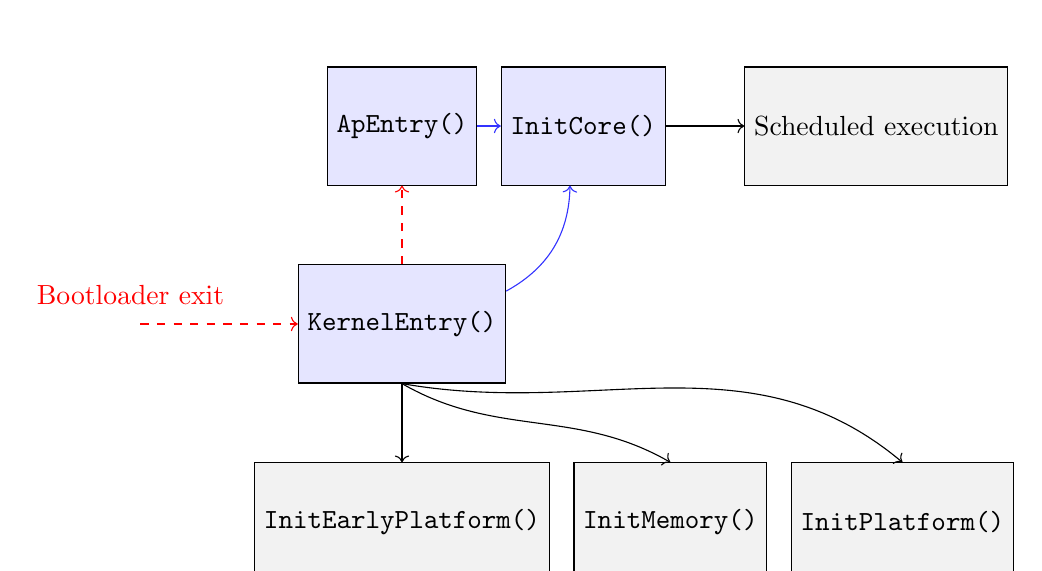
\begin{tikzpicture}
    \node (ApEntry) [rectangle, minimum height=1.5cm, draw=black, fill=blue!10] {
        \verb|ApEntry()|};
    \node (KernelEntry) [rectangle, minimum height=1.5cm, draw=black, fill=blue!10, below = of ApEntry] {
        \verb|KernelEntry()|};
    \node (hidden) [left = 2cm of KernelEntry] {};
    \node (InitCore) [rectangle, minimum height=1.5cm, draw=black, fill=blue!10, right = 3mm of ApEntry] {
        \verb|InitCore()|};
    \node (SchedulerExec) [rectangle, minimum height=1.5cm, draw=black, fill=gray!10, right = of InitCore] {
        Scheduled execution
    };
    \node (InitEarlyPlatform) [rectangle, minimum height=1.5cm, draw=black, fill=gray!10, below = of KernelEntry] {
        \verb|InitEarlyPlatform()|};
    \node (InitMemory) [rectangle, minimum height=1.5cm, draw=black, fill=gray!10, right = 3mm of InitEarlyPlatform] {
        \verb|InitMemory()|};
    \node (InitPlatform) [rectangle, minimum height=1.5cm, draw=black, fill=gray!10, right = 3mm of InitMemory] {
    \verb|InitPlatform()|};

    \path [->, red, dashed] (hidden) edge (KernelEntry.west) node [label=above:Bootloader exit]{};
    \path [->] (KernelEntry.south) edge (InitEarlyPlatform);
    \path [->, in=150, out=-30] (KernelEntry.south) edge (InitMemory.north);
    \path [->, in=140, out=-10] (KernelEntry.south) edge (InitPlatform.north);
    \path [->, red, dashed] (KernelEntry) edge (ApEntry);
    \path [->, bend right, blue!80] (KernelEntry) edge (InitCore);
    \path [->, blue!80] (ApEntry) edge (InitCore);
    \path [->] (InitCore) edge (SchedulerExec);
\end{tikzpicture}

\centering
\begin{tabular}{c|c|l}
    \begin{tikzpicture}
        \path [->, red, dashed] (0, 0) edge (1, 0);
    \end{tikzpicture} 
    & 
    & Platform-specific mechanism. \\

    \begin{tikzpicture}
        \path [->, blue!80] (0, 0) edge (1, 0);
    \end{tikzpicture} 
    & 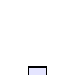
\begin{tikzpicture} \node (r)[rectangle, draw=black, fill=blue!10] (0, 0){}; \end{tikzpicture} 
    & (Call to) platform specific code. \\

    \begin{tikzpicture}
        \path [->, black] (0, 0) edge (1, 0);
    \end{tikzpicture} 
    & 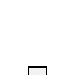
\begin{tikzpicture} \node (r)[rectangle, draw=black, fill=gray!10] (0, 0){}; \end{tikzpicture}
    & (Call to) common init code. \\
\end{tabular}
\caption{Kernel operation pre-scheduler.}
\end{figure}

\subsection{Multi-Core Systems}
The kernel is written and tested with multi-core systems in mind, but it's also capable of running on single-core systems. 

From the perspective of the kernel, each core operates independently of the others. The majority of the kernel subsystems are unaware of how many cores are present in the system. The scheduler and IPI mailboxes are the notable exceptions, as they operate on a per-core basis. The scheduler is covered in more in \autoref{Scheduler}.

During initialization one core is considered the boot core (the BSP, to use the x86 term) and will set up the initial memory management structures used for the kernel, and perform other early init operations like discovering and initializing early log outputs (like serial devices or the bootloader framebuffer). The boot core is also responsible for starting the other cores in the system so they can initialize themselves. Once each core has finished initializing itself, it will begin scheduled execution. 

At runtime one core is given the special duty of managing the system clock. This is often the boot core, but is not required to be. The clock core is responsible for managing the hardware timer(s) used to provide the clock functions to the rest of the kernel.

If for some reason a function is required to run on a specific core, there are two options:
\begin{itemize}
    \item A thread can be created to run the function, and pinned to a specific core. This is the recommended approach for code without timing requirements.
    \item Each core has an IPI mailbox. Each mail item consists of a function pointer and an argument to pass to the function when run. When mail is sent the target core is sent an IPI and the function will whenever the IPI is served. See the function \verb|SendIpiMail()| in \verb|interrupts/Ipi.h|.
\end{itemize}

\subsubsection{Example Code}
To use the mailbox mechanism all that's required a pointer to the function to run on the remote core. In the example we'll assume core 5 exists and we want to run \verb|ExampleFunction()| on that core. The callback function can optionally have an argument passed to it at runtime, but it's not required so we'll use \verb|nullptr|. We omit the argument in this example. The function we'll use is defined in \verb|interrupts/Ipi.h|.

\begin{verbatim}
void ExampleFunction(void* ignored);

SendIpiMail(5, ExampleFunction, nullptr);
\end{verbatim}

\section{Supported Platforms}
This version of the kernel was written with support for multiple platforms in mind from the beginning, and it was one of the earliest features of the kernel. Currently only two platforms are supported (x86\_64 and riscv64) but it would be nice to add more in the future, namely aarch64 and perhaps something more exotic.

The current platforms and their status are listed below.

\begin{tabular}{|r|l|p{0.3\linewidth}|p{0.4\linewidth}|}
    \hline
    \textbf{Platform} & \textbf{Qemu} & \textbf{Hardware} & \textbf{Notes} \\
    \hline
    x86\_64 & Yes & 3 machines tested, 2 work. & \\
    riscv64 & Yes & No & Support for a visionfive-2 port is planned once some bugs are ironed out in the virtio machine.\\
    \hline
\end{tabular}

\subsection{Platform Abstraction Layer}
The kernel maintains a strict boundary between platform-specific code and platform-independent code. The platform specific code is contained within the \verb|kernel/arch/xyz| and \verb|kernel/include/arch/xyz| directories, where \verb|xyz| is the target architecture. Each platform is given it's own directory, and the layout inside this directory can be considered freeform.

Each platform \textbf{must} implement the functions defined in each header file under \verb|kernel/include/arch|. These headers contain functions required by the rest of the kernel. Code within an arch directory is allowed to include headers from within it's own \verb|include/arch/xyz/| directory, however all other kernel code is only permitted to use the generic headers found in \verb|include/arch/|.

\subsubsection{Platform.h}
This file is a special case, as the platform agnostic \verb|kernel/include/arch/Platform.h| provides some complete definitions (like the core-local data struct), some utility functions and also some function declarations. These declarations serve as a guide for what a platform would need to implement to support a port of the kernel. 

Most of the declared functions can be implemented by simple inline assembly, and often these functions are made \verb|inline| (often with \verb|[[gnu::always_inline]]| too). There are some additional constants that must be defined within an implementation of this header:

\begin{itemize}
    \item \verb|size_t PageSize|: The native page size of the target platform, in bytes. Most platforms will have this as 4K (0x1000) bytes.
    \item \verb|size_t IntVectorAllocBase|: Used by the interrupt vector allocator, this sets the lowest vector number available for general use. Vectors will never be allocated below this.
    \item \verb|size_t IntVectorAllocLimit|: Largest interrupt vector allowed to be allocated (inclusive). Set this and \verb|IntVectorAllocBase| to 0 to disable the vector allocator and the ability to install interrupt handlers.
\end{itemize}

Of course platforms are free to define their own internal constants here too, for example x86\_64 defines a number of MSR and port values.

\subsection{Platform Requirements}
The northport kernel is inteded to run on mobile or desktop class processors, and currently there is no intent to support embedded processors.

The hardware requirements for adding a new platform are described below.

\begin{itemize}
    \item An MMU for managing the virtual address space, with the ability to distinguish between supervisor and user levels, and r/w/x access control.
    \item Basic interrupt architecture: sending device interrupts to specific processors, or at least limiting which processors can receive them. The ability to send IPIs is also required on multi-core systems.
    \item A single timer capable of sending an interrupt on a terminal count (one-shot operation), and a timer that can be used for polling. There are no strict timing requirements, but the kernel internally tracks time as nanoseconds, and so it can make use of more precise timers if available. The kernel doesn't care if these two functions are provided by the same piece of or hardware or two separate pieces. Only one of each type of timer is needed, and they both need to be accessible from the same processor. The system must provide a way to calibrate each timer.
    \item The kernel expects to be booted in accordance with the Limine Boot Protocol. If a compatible bootloader exists for the target platform that's easy, but if not the boot shim included in the kernel may need to be modified.
\end{itemize}

The kernel also has a soft requirement of being running on a 64-bit processor. Although it should be possible to port to a 32-bit system, this isn't a goal of the project and is yet to be tested.

\section{Physical Memory Manager}
The kernel uses a relatively simple physical memory manager design, with a focus on keeping allocations fast and using granular locking to reduce contention between multiple cpus trying to allocate at the same time.

A bitmap allocator is not the fastest, but it is accountable. This is an important feature in the PMM design: bad attempts to free physical memory won't result in corrupt state. While other allocator designs can offer this, a bitmap is simple to implement.

\subsection{Concepts}
\paragraph{PM Zone}
Zones are used to arbitrarily section-off parts of physical memory. In northport two zones are used: the low zone (32-bit addressable memory), and the high zone (addresses > 4GiB).
This is done in an attempt to preserve 32-bit addressable memory for older devices that only support these 32-bit addresses. While these devices are less common, they are not extinct.

\paragraph{PM Range}
A range represents a number of contiguous physical pages, and tracks the state of each page (used/free) in a bitmap. A range also contains some metadata like where the next free page is, the total number of free and used pages, etc. Each range is responsible for a fixed number of pages, but the PMM's view of physical memory can be modified by adding or removing ranges.

As the ideas of a range or zone are used elsewhere in the kernel, these are referred to as \textbf{PM}Ranges or \textbf{PM}Zones to indicate they represent physical memory.

\begin{figure}[h]
\centering
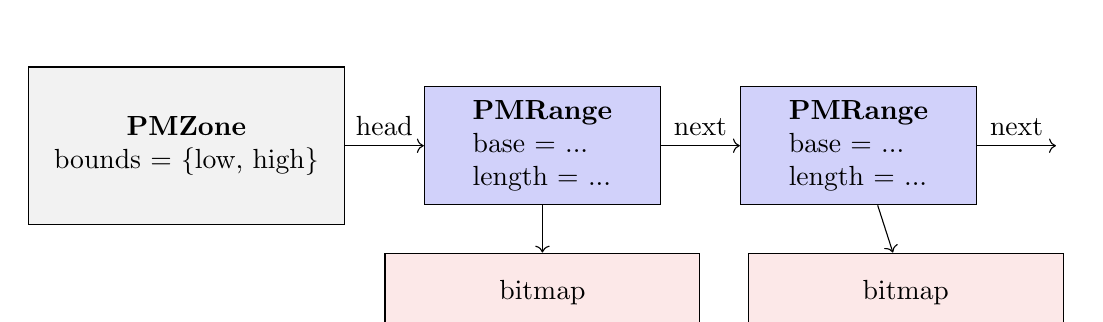
\begin{tikzpicture}
    \begin{scope}
    \node (1) [rectangle, minimum width=3cm, minimum height=2cm, draw=black, fill=gray!10] {
        \begin{tabular}{c}
            \textbf{PMZone} \\
            bounds = $\lbrace$low, high$\rbrace$
        \end{tabular}};
    \node (2) [rectangle, minimum width=3cm, minimum height=1cm, draw=black, fill=gray!20!blue!20, right = of 1] {
        \begin{tabular}{l}
            \textbf{PMRange} \\
            base = ... \\
            length = ... \\
        \end{tabular}};
    \draw [->] (1) -- node[above] {head} (2);
    \node (3) [rectangle, minimum width=3cm, minimum height=1cm, draw=black, fill=gray!20!blue!20, right = of 2] {
        \begin{tabular}{l}
            \textbf{PMRange} \\
            base = ... \\
            length = ...
        \end{tabular}};
    \draw [->] (2) -- node[above] {next} (3);
    \node (4) [right = of 3] {};
    \draw [->] (3) -- node[above] {next} (4);
    \end{scope}
    \begin{scope}[node distance=6mm]
        \node (bitmap0) [rectangle, minimum width=4cm, minimum height=1cm, draw=black, fill=gray!20!red!10, below = of 2] {bitmap};
        \node (bitmap1) [rectangle, minimum width=4cm, minimum height=1cm, draw=black, fill=gray!20!red!10, right = of bitmap0] {bitmap};
        \draw [->] (2) -- (bitmap0);
        \draw [->] (3) -- (bitmap1);
    \end{scope}
\end{tikzpicture}
\caption{Relationship between PMZones and PMRanges.}
\end{figure}

\begin{figure}[h]
\centering
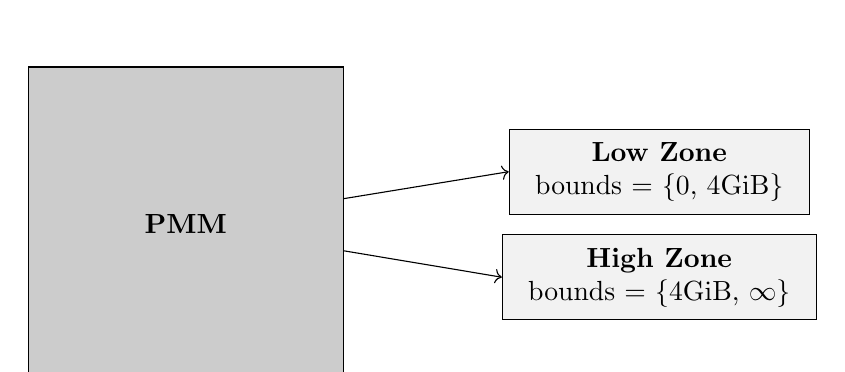
\begin{tikzpicture}
    \node (pmm) [rectangle, minimum width=4cm, minimum height=4cm, draw=black, fill=gray!40] {
        \textbf{PMM}
    };
    \node (placeholder) [minimum width=4cm, minimum height=0cm, right = 2cm of pmm]{};
    \node (lowzone) [rectangle, minimum width=2cm, minimum height=1cm, draw=black, fill=gray!10, above = 0mm of placeholder] {
        \begin{tabular}{c} 
            \textbf{Low Zone} \\
            bounds = $\lbrace$0, 4GiB$\rbrace$
        \end{tabular}
    };
    \node (highzone) [rectangle, minimum width=2cm, minimum height=1cm, draw=black, fill=gray!10, below = 0mm of placeholder] {
        \begin{tabular}{c} 
            \textbf{High Zone} \\
            bounds = $\lbrace$4GiB, $\infty\rbrace$
        \end{tabular}
    };
    \draw [->] (pmm) -- (lowzone.west);
    \draw [->] (pmm) -- (highzone.west);
\end{tikzpicture}
\caption{PMM zone configuration.}
\end{figure}

\subsection{Initialization}
The northport PMM uses a bitmap to store the state of page of physical memory. A page is considered the basic unit of the PMM, and it's exact size depends on the target platform and is represented by the constexpr variable \verb|PageSize|.

The first problem the PMM is presented with is finding space for the bitmaps required to manage each region. For memory effeciency these bitmaps are packed together, since the next bitmap can begin inside of the slack space following the previous bitmap. This slack space refers to the space following the end of the bitmap, but before the next page begins. Since the PMM operates in page-sized units, this space is wasted.

The downside to this approach is that a single large space is required for the bitmaps to exist in, rather than many smaller spaces. This is fine on most systems, but may break down on a sufficiency fragmented physical memory map.

The buffer used for the bitmaps is called the \textit{metabuffer} and is also used for allocating the space needed for the PM regions. Each PM region roughly represents a single usable memory map entry. Once the space required for the metabuffer has been calculated, it's length is rounded up to the nearest page and subtracted from the largest memory map entry available before having the hhdm offset added.

The address and length of the metabuffer is stashed, and the PMM begins ingesting each usable memory region from the memory map.

\subsection{Ingesting Memory}
Ingesting physical memory makes it available for use by the rest of the system. Memory can be ingested at any time, although this can become a very expensive operation once more processes are started. While adding memory at runtime is supported, removing memory from the system is currently not.

When memory is ingested it may be split into two separate regions if it crosses a PM zone border. Otherwise the ingested memory is represented by a single PM region. 

The PM regions and their bitmaps are allocated from the metabuffer. Each region is the inserted into the linked list of regions representing the PM zone it's assigned to. This list is sorted by base address (ascending).

At this point the new PM region is live and can be accessed by the rest of the PMM, and can now be used to satify allocations.

\subsection{Allocating Pages}
Allocating memory is very straightforward, each PM region tracks how many free pages it contains. If the region lacks enough free pages to satisfy an allocation request, it's skipped.

Once a region with enough free pages is found, the region's bitmap is scanned until a run of contiguous free pages is found. If this run is not found, the search for a new region with enough free pages continues.

If an allocation request cannot be satisified, the PMM panics the kernel. There are plans to allow the PMM to communicate memory pressure to users of physical memory and request to purge some allocations, allowing physical memory to freed to satisfy other allocations. This (and some other ideas) currently only exist as experiments.

It should be noted that there are two main allocation functions:
\begin{itemize}
    \item \verb|AllocLow()|: This function tries to allocate exlusively from the low zone (< 4GiB), and panics on failure.
    \item \verb|Alloc()|: This function tries to allocate from the higher zone, and on failure calls \verb|AllocLow|. Ultimately this may cause a panic on failure.
\end{itemize}

The intention is for developers to use \verb|Alloc| for general physical memory allocations, and only use \verb|AllocLow| for memory that must be 32-bit addressable.

\subsection{Freeing Pages}
Freeing memory is also straightforward. First the appropriate zone for the allocation is selected, and then the freed address is compared against the base address and length of each PM region in the zone until the matching region is found. If the zone or region could not be determined, an error is logged and the freeing call fails. In this event no bitmap state is modified.

Once the PM region has been located, the corresponding bit is cleared, and the free operation is complete.

Contrary to allocation, there is only a single free function \verb|Free()|.

\subsection{Example Code}
The PMM operates as a singleton, and the global instance is available as \verb|PMM::Global()|. The alloc/free functions will assume a page-count of 1 unless otherwise specified. All the functions used below are declared in \verb|memory/Pmm.h|.

\begin{lstlisting}
uintptr_t singlePage = PMM::Global().Alloc();
uintptr_t sixPages = PMM::Global().Alloc(6);

PMM::Global().Free(singlePage);
PMM::Global().Free(sixPages, 6);
\end{lstlisting}

\section{Virtual Memory Manager}
The virtual memory subsytem takes inspiration from a paper on the old SunOS VMM design: where the subsystem is composed of a few distinct parts:

\begin{itemize}
    \item The VMM itself acts as a high level manager of an address space. It's responsible for tracking and allocating in-use/free virtual addresses and their associated permissions. However it's not responsible for managing the backing memory behind virtual memory it manages, this is the responsibility of the associated VM driver.
    \item A number of VM drivers, which act as plugins to a VMM. Each VM driver is responsible for a certain type of backing that is \textit{attached} to virtual memory allocated by the VMM. A driver can be thought of as 'glue code' between virtual memory and physical memory being used for a particular purpose. See \autoref{vmdrivers} for specifics.
    \item All of this operates on top of the \textit{HAT} (hardware address translation), a term borrowed from other kernels. The HAT is part of the arch layer of the kernel, and represents an abstract memory management unit. Any supported architectures must provided a HAT implementation, which allows the VMM and VM drivers to communicate with the underlying hardware. The use of this layer allows the rest of the virtual memory subsystem to remain completely platform independent and portable.
\end{itemize}

TODO: add lines showing separation between layers of arch, subsystem and them VMOs on top (expected API).

\begin{figure}[h]
\centering
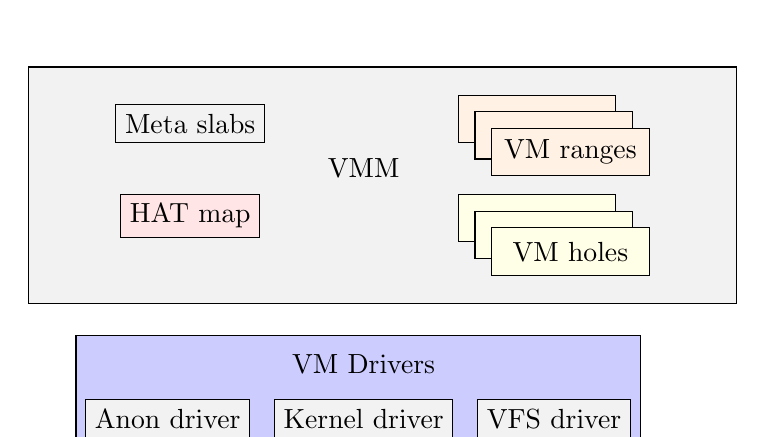
\begin{tikzpicture}
    \node (vmm) {VMM};
    \node (mgmtanchor) [right = 1.5cm of vmm] {};
    \node (metaanchor) [left = 1.5cm of vmm] {};

    \node (vmrange0) [rectangle, minimum width=2cm, minimum height=0.6cm, draw=black, fill=orange!10, above = 2mm of mgmtanchor] {};
    \node (vmrange1) [rectangle, minimum width=2cm, minimum height=0.6cm, draw=black, fill=orange!10, below right = 3mm of vmrange0.north west] {};
    \node (vmrange2) [rectangle, minimum width=2cm, minimum height=0.6cm, draw=black, fill=orange!10, below right = 3mm of vmrange1.north west] {VM ranges};

    \node (vmhole0) [rectangle, minimum width=2cm, minimum height=0.6cm, draw=black, fill=yellow!10, below = 2mm of mgmtanchor] {};
    \node (vmhole1) [rectangle, minimum width=2cm, minimum height=0.6cm, draw=black, fill=yellow!10, below right = 3mm of vmhole0.north west] {};
    \node (vmhole2) [rectangle, minimum width=2cm, minimum height=0.6cm, draw=black, fill=yellow!10, below right = 3mm of vmhole1.north west] {VM holes};

    \node (metaalloc) [rectangle, draw=black, fill=gray!10, above = 2mm of metaanchor] {Meta slabs};
    \node (hatmap) [rectangle, draw=black, fill=red!10, below = 2mm of metaanchor] {HAT map};

    \node[rectangle, minimum width = 9cm, minimum height = 3cm, draw=black, fit=(vmm) (vmrange0) (vmrange2) (vmhole0) (vmhole2) (metaalloc)] {};

    \node (vmdrivers) [below = 2cm of vmm] {VM Drivers};
    \node (vmdriver0) [rectangle, draw=black, fill=gray!10, below = 2mm of vmdrivers] {Kernel driver};
    \node (vmdriver1) [rectangle, draw=black, fill=gray!10, right = 3mm of vmdriver0] {VFS driver};
    \node (vmdriver2) [rectangle, draw=black, fill=gray!10, left = 3mm of vmdriver0] {Anon driver};
    \node [rectangle, draw=black, fit=(vmdrivers) (vmdriver0) (vmdriver1) (vmdriver2)] {};

    \begin{scope}[on background layer]
        \node[fill=gray!10, minimum width = 9cm, minimum height = 3cm, fit=(vmm) (vmrange0) (vmrange2) (vmhole0) (vmhole2) (metaalloc)] {};
        \node[fill=blue!20, fit=(vmdrivers) (vmdriver0) (vmdriver1) (vmdriver2)] {};
    \end{scope}
\end{tikzpicture}
\caption{The various components of the virtual memory subsystem.}
\end{figure}

\begin{figure}[h]
\centering
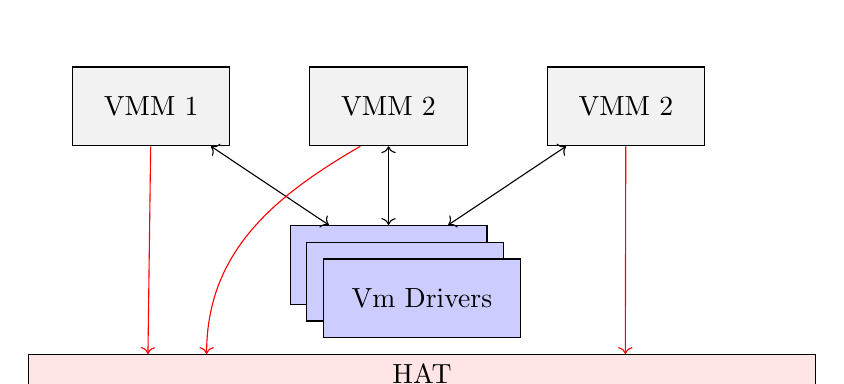
\begin{tikzpicture}
    \node (vmm1) [rectangle, minimum width=2cm, minimum height=1cm, draw=black, fill=gray!10] {VMM 1};
    \node (vmm2) [rectangle, minimum width=2cm, minimum height=1cm, draw=black, fill=gray!10, right =of vmm1] {VMM 2};
    \node (vmm3) [rectangle, minimum width=2cm, minimum height=1cm, draw=black, fill=gray!10, right =of vmm2] {VMM 2};

    \node (vmdriver1) [rectangle, minimum width=2.5cm, minimum height=1cm, draw=black, fill=blue!20, below = of vmm2] {};
    \node (vmdriver2) [rectangle, minimum width=2.5cm, minimum height=1cm, draw=black, fill=blue!20, below right=3mm of vmdriver1.north west] {};
    \node (vmdriver3) [rectangle, minimum width=2.5cm, minimum height=1cm, draw=black, fill=blue!20, below right=3mm of vmdriver2.north west] {Vm Drivers};

    \node (hat) [rectangle, minimum width=10cm, minimum height=5mm, draw=black, fill=red!10, below= 2mm of vmdriver3] {HAT};

    \draw [<->] (vmm1) -- (vmdriver1);
    \draw [<->] (vmm2) -- (vmdriver1);
    \draw [<->] (vmm3) -- (vmdriver1);

    \node (hat0) [minimum height=5mm, right = 1.4cm of hat.west] {};
    \node (hat1) [minimum height=5mm, right = 5mm of hat0] {};
    \node (hat2) [minimum height=5mm, left = 2.3cm of hat.east] {};
    \node (vmm2fudge) [rectangle, minimum width=5mm, minimum height=1cm, left =1mm of vmm2.center] {};

    \draw [->, red] (vmm1) -- (hat0);
    \path [->, in=90, out=210, red] (vmm2fudge.south) edge (hat1);
    \draw [->, red] (vmm3) -- (hat2);
\end{tikzpicture}
\caption{Relationship between multiple VMMs, VM drivers and the HAT.}
\end{figure}

\subsection{Concepts}

\paragraph{VM Range}
Used internally by the virtual memory subsystem to represent a range of virtual addresses. It contains the usual base and length, as well some flags to store what the memory should be able to do. It also contains an offset field as the virtual address returned may not always point to the start of the VM range. This is to allow things like the VMM adding guard pages to the range, which are included as part of the VM range but not included in the virtual memory made available to the consumer. This also allows for virtual memory to map things in ways that might be misaligned according to the MMU, as the offset provides a byte sized granularity. Each range also contains a \verb|token| field, which holds an opaque pointer for the VM driver that is attached to this range.

\paragraph{VM Driver} 
\label{vmdrivers}
While these are called VM \textit{drivers} they have nothing to do with the device driver subsystem, and are loaded much earlier than that. It might be more accurate to think of them as plugins to the VMM, with each one providing one type virtual memory that can be used for VM ranges.

\begin{itemize}
    \item Anon VM Driver: Provides general purpose 'working memory'. This is the most common type of virtual memory and ultimately just allocates physical memory and maps it where appropriate. This driver makes heavy use of the page fault handler to perform operations like demand paging and a primitive form copy-on-write.
    \item VFS VM Driver: Acts as a bridge between the VMM and the VFS, and allows for mapping the contents of a file into an address space. It has full support for demand paging, and can trigger parts of a file to be loaded from disk if they are not present in the file cache.
    \item Kernel VM Driver: This driver is a catch-all for all the other operations the kernel might need to perform on virtual memory. This driver is responsible for making sure the kernel binary is mapped properly in virtual memory, and at runtime it can be used to map MMIO (physical addresses that aren't usable memory) into an address space.
\end{itemize}

\paragraph{Virtual Memory Object}
A \textit{virtual memory object} (VMO) is a wrapper around a VM range and the VMM that owns it. The intention is to provide a cleaner interface than the VMM itself provides, and to abstract the complexity exposed by the VMM. The full API is still available if needed, but for the vast majority of use cases a VMO has the required features. As such, the VMO is the recommended way to manage virtual memory, it also makes use of RAII to help prevent leaks. VMOs can also be freely passed around the kernel as a way to represent 'some memory in an address space'.

\subsection{Hardware Abstraction}
The VMM and VM drivers are written to be independent of the underlying hardware, instead relying on the HAT (\textit{hardware address translation} - a borrowed term) to access the hardware. The HAT is part of the arch-layer of the kernel, and acts as the interface to the the platform's MMU.

The HAT makes use of a few primitives, namely \textit{modes} and \textit{maps}. A mode describes one possible way that the MMU can map memory, specifying an alignment and granularity. Modes and and the number of them available are collectively referred to as the \textit{HAT limits}. A map is an opaque representation of an address space. From the kernel perspective a map is an opaque pointer, and the VMM will store exactly one of these per managed address space. In systems using paging, the map is usually the root page table. The HAT also provides a handful of functions for managing mappings within an address space.

The VMM and VM drivers make full use of the available modes exposed by the HAT, meaning that the limitations placed on virtual memory management are based on what the hardware supports - no artificial limits are imposed by the VMM.

\subsection{Address Space Management}
TODO: ranges list, holes list, use of list vs tree (list is easier to conceptualize - tree for speedy runtime).
Cover alloc + free.

\subsection{Kernel VMM}
TODO: vs lower half user vmms

\subsection{Initialization}
Immediately after the physical memory manager is initialized, the kernel VMM is brought up. First \verb|HatInit()| is called, which allows the architecture layer to perform some global setup, as well as map the HHDM in the map used by the kernel VMM. The reason the HAT is responsible for mapping the HHDM instead of the VMM is that the HAT can freely make assumptions about the best way to map the large, continuous area of address that the HHDM occupies. This function is only called once and is therefore not suitable for core-local setup of the MMU. It's mainly for detecting what mode the MMU is in (e.g. how many paging levels are available and in use), and any optional extensions. Next the VM drivers are initialized, this mainly consists of detecting and setting some software feature flags. The exception here is the kernel VMM which maps the kernel binary with (propoer permissions) into the address space of the kernel VMM.

It should be noted that at this point the kernel is still running using the MMU settings setup by the bootloader. The next step is the actually initialize the kernel VMM instance by telling it what range of addresses it has available: these start immediately after the HHDM and end just before the kernel binary begins. At this point the kernel VMM switches loads it's own address map.

The kernel VMM also instructs the global kernel heap to initialize itself at this point, however this is detailed in \autoref{Heap}.

\subsection{Address Space Management}
Both active VM ranges and free space are organised in similar ways: each instance is represented by a struct storing the base address and length, and these structs are stored in a red-black tree. Originally a singly-linked list was used for tracking active VM ranges, but this doesn't scale well with large numbers of ranges. A binary tree was a better option and a red black tree had desirable characteristics, although the major downside is the amount of code and complexity it adds to the kernel. In the future this may be replaced with an andersson (AA) tree to reduce this complexity a little.

The tree of free addresses (referred to as \textit{holes}) represents what parts of the address space are free for allocations, while another tree (\textit{ranges}) stores the structs holding information about active VM ranges. While not used anywhere in the code, there is a soft concept of an inactive VM range, which is space not stored in either tree: i.e. its not allocatable but does isn't accessible to the rest of the system. Currently this is not supported or implemented, but this idea may be revisited in the future.

\subsection{Meta Allocators}
Allocating memory for the VM ranges and address space hole structs can't be done via the global kernel heap, as the heap is built on top of the virtual memory subsystem. To avoid this circular dependency, a VMM also contains a number of slab allocators known as \textit{meta allocators}. Each slab is sized around one type of metadata struct that needs to be stored: one slab for VM ranges, one for VM holes. Internally these allocators are quite simple, consisting of a linked list of individual slabs accompanied by a bitmap tracking a slab's free/in-use status.

The backing memory for these slabs are allocated directly from the PMM, and then these are accessed via the HHDM. This means the memory used for these allocators is managed outside the heap and virtual memory stacks and don't gain the benefits afforded by either of them (e.g. demand paging or CoW).

\subsection{Allocation}
There's a few key steps to allocating a new chunk of virttual memory. First the VMM finds the correct VM driver for the type of memory requested via the \verb|flags| argument. Then the VMM calls \verb|vmdriver.Query()| to determine exactly how much space is needed for the allocation and the required alignment. The VM driver might require more space for the allocation than was requested depending on the limits exposed by the HAT. For example if mapping a file via the VFS VM driver with an offset of 123 bytes, which is not aligned with the HAT mode chosen by the file cache. The VM driver would need to start mapping the VM range at the nearest address aligned to the chosen HAT mode, and then return a pointer 123 bytes beyond the start of the mapping.

\begin{figure}[h]
\centering
\caption{Example usage of the VM range offset field when mapping a file.}
\end{figure}

This mechanism of returning an offset into the allocated VM range also easily allows for other mechanisms like guard pages.

\begin{figure}[h]
\centering
\caption{Using the offset field for Guard Pages.}
\end{figure}

After calling \verb|Query()| on the VM driver, the VMM finds an appropriate area of unused address space for the VM range to occupy, and creates a new VM range struct. The free space is marked as in-use and the VM range struct is populated with details like the base address and length of the range.

At this point the VMM calls \verb|vmdriver.Attach()| which is where the VM driver begins managing the mappings associated with the VM range. Note that the driver isn't required to actually map anything yet, depending on it's configuration. It may wait for the VMM to signal a fault before committing any physical memory or other resources. During this function the VM driver can return a \textit{token}, which acts as a private pointer between the range and the VM driver. This token is stored in the VM range struct, and is available to the driver any time it's requested to oeprate on the VM range.

Once the VM driver is attached, the range is inserted in the \verb|ranges| tree and is now considered active.

\subsection{Usage of Page Faults}
The VMM and VM drivers make full usage of page faults (and handling them). Often a fault is triggered by the hardware in response to action taken by a program, but a page fault can also be triggered manually by calling \verb|HandleFault()| on any VMM to trigger the same response. This function returns a bool indicating if the fault was considered 'good' or not. A good fault is an allowed (and expected) memory access, while a bad fault is an illegal one.

Bad faults can result in any number of consequences, from a program being terminated to a kernel panic, depending on the VMM in question.

When handling a page fault the VMM will check the faulting address against the list of active VM ranges, looking for the associated range. If a matching range isn't found, the fault returns \verb|false| as it failed to handle it properly. If the range is found, the VMM will then check the fault flags which describe what the memory access was (read, write or execute), it's privilege level (supervisor or user). Assuming the memory access was allowed for this VM range, the VMM will call the fault handler on the VM driver attached to the range and allow the driver to continue handling the fault. At this point the VM driver is responsible for the outcome of the fault.

VM drivers may choose to not map physical memory with the full permissions requested by the VMM, in order to trigger a fault on certain actions. This is used to implement features like CoW (copy-on-write), zero-paging, or to allow the backing memory to be reclaimed and used elsewhere. \textit{Current swapping to disk isn't implemented, and the file cache is only half transient - it has no page-out features}

At this point the action taken depends on the specific VM driver and the exact nature of the fault.

\subsection{Example Code}

\section{Heap Allocation}
The kernel heap is provided by a series of aggregate slab allocators and a pool allocator. All of this is hidden behind the heap API, which consists of familiar free/alloc functions, and the C-style \verb|malloc()| and \verb|free()| global functions are provided as well (see \verb|memory/New.cpp|) if they're needed. The C functions are simple wrappers around the main heap functions.

The global \verb|new| and \verb|delete| C++ operators have also been defined, making them available for kernel code. This is the ideal way to manage dynamically allocated memory.

\subsection{Concepts}

\paragraph{Pinned Allocations} By default the kernel heap uses memory that can be swapped (purged from main memory to disk to free memory for use parts of the system) and demand-paged. Allocations can optionally be made \textit{pinned}. Pinned allocations are immediately backed with physical memory and non-swappable, which is useful for critical parts of the kernel infrastructure that can't be swapped out. The container used by the VMM to track allocated VMRanges is an example of when pinned memory is needed. Pinning allocations means that the physical memory used can't be used elsewhere if the system needs it, so they should be used sparingly and only when necessary.

\subsection{Slab Allocators}
For small heap allocations the kernel uses a series of slab allocators, with each slab being 2x the size of the pervious. The smallest slab allocator starts at 32 bytes, and the largest is 512 bytes by default, although this is easily configurable. 

Each slab consists of a number of \textit{slab segments}, which contains a base address and bitmap to track which slabs have allocated relative to the base. A segment also contains some extra metadata to speed up allocations, like hinting at where the last successfull allocation was.

When a segment is full, a new segment is created with identical parameters to the initial segment (slab size and number of slabs). These segments are stored as a linked list, effectively allowing infinite expansion if needed. As each slab tracks the number of free slabs, full segments can quickly be skipped when searching for free space.

\subsubsection{Pinned vs Non-Pinned}
Each slab allocator also tracks if it's pinned or not. Non-pinned slabs operate as you would expect, but pinned slabs are a special exception in how virtual memory is managed in the kernel. There is a circular dependency between pinned slabs and the VMM: since the VMM uses pinned allocations to store its management structures, the slab cannot use the VMM to allocate more virtual address space for itself as this would cause a pinned allocation, and so on. 

The current solution is to reserve an area of virtual memory above the HHDM but below the area the kernel VMM is allowed to allocate in. This area is the same size as the HHDM. A pointer within this area is stored, and is treated like a bump allocator: everytime a pinned slab expands it increments this pointer by the amount of virtual memory the new segment will consume. When it comes to back the new segment with physical memory, the slab modifies the kernel's master page tables directly.

\subsection{Pool Allocators}
The pool allocator is similar to the design of \hyperlink{https://github.com/blanham/liballoc}{liballoc} v1.1. It consists of a number of segments, and each segment is a freelist for a single contiguous block of virtual memory. Over time as the pool allocator expands more segments may be added. 

There are no major differences between the pinned pool vs the non-pinned pool, except for the flags passed to the VMM when requesting virtual memory. The VMM handles the specifics of pinning memory.

\subsection{Example Code}
Like other singleton classes the global kernel heap can be accessed as \verb|Heap::Global()|. All heap declarations are available in the header \verb|memory/Heap.h|. The examples below are for documentation but the built-in C++ operators should be used where possible.

\begin{verbatim}
void* _100Bytes = Heap::Global().Alloc(100);

Heap::Global().Free(_100Bytes);
\end{verbatim}

To use pinned allocations is similar, although you must tell \textit{both} alloc and free that this is pinned memory. This can be done by setting the optional argument to \verb|true|. A \verb|PinnedAllocator| class is also available for use as the allocator argument in template containers.

\begin{verbatim}
void* _40BytesPinned = Heap::Global().Alloc(40, true);

Heap::Global().Free(_40BytesPinned);        //an error
Heap::Global().Free(_40BytesPinned, true);  //okay
\end{verbatim}

\section{Clocks and Timers}
Northport refers to hardware devices that provide timekeeping facilities as timers, and provides a software abstraction on top called a clock. There is only one clock in the system, and the rest of the kernel uses the clock for getting timer callbacks. Internally the clock uses whatever timers are provided by the platform to ensure it can keep the deadlines set by software.

It's important to note that the timing subsystem is 'best-effort' and \textbf{not real time}. Clock events are guarenteed to expire \textit{exactly once}, and \textit{reasonably soon} after their ideal expiry time. Reasonably soon is relative to the accuracy and precision of the hardware timers being used to drive the clock.

\subsection{Hardware Timers}
Northport has very simple timing requirements, this was done with the intent of making the kernel easier to port to other platforms. There are two types of timers we require, although only one of each is necessary.

\paragraph{Polling Timers}
A polling timer only needs to provide a software readable counter. The kernel assumes values returned from the counter increment as time passes, regardless of what the underlying timer does. If the timer counts down, you can return the inverted value (\verb|maxCount - currentCount|). The x86 PIT is one such example, which counts down: and when used for the system polling timer the returned value is inverted so the system sees an incrementing value.

\paragraph{Interrupt Timers}
Interrupt timers require the ability to set a deadline in the future, and generate an interrupt whenthe deadline is passed. Deadlines are often within the 1-1000ms range, but the kernel can take advantage of hardware that supports longer expiry times. Interrupt timers may also be referred to as \textit{sys timers} in the source code (the original term used).

The kernel doesn't interact with the various timers directly, instead it uses the functions defined in \verb|arch/Timers.h| to interface with platform specific code that manages the underlying hardware. Anything beyond the functions in that header are considered implementation details of the platform. This includes calibrating any timers that might require it.

\subsection{Software Clock}
The clock is the main timing interface for the kernel. It works by keeping a list of pending \textit{clock events}. This list is sorted with the soonest event at the head of the list, and each event tracks it's time relative to the previous event. The interrupt timer is set to the first event in the list, and the event's callback function runs is called in response to the timer expiring. The time taken for each callback to run is tracked, and any pending events that would have expired in that time are also run.

It's important to note that the callback handler runs inside the interrupt handler. Recommended practice is to queue a DPC to perform as much of the work as possible rather than running inside the interrupt handler.

In a multicore system the clock is managed by whichever core manages the hardware timers. This is usually the first core to boot (the BSP). The clock ensures that callbacks always run on the core they were queued from, regardless of which core manages the clock. For cores other than the BSP the callback is executed via the IPI mailbox mechanism.

\paragraph{Infinite Expiry Times}
If a clock event is set to expire at a time too far away for the hardware clock to encode, \textit{virtual clock events} are inserted at the clock's longest expiry time until the original event expiry time is reachable. This trades total clock duration for a little bit of memory, but allows for near-infinite expiry times (memory permitting).

\subsection{Platform Specific Details}

\subsubsection{X86}
X86 has a large number of timers available. We try the most useful timers first, and fall back to known-good timers if those fail or are not available. The timers are sourced in the following orders:

\textbf{Polling timer:} TSC, HPET main counter, PIT counter.\\
\textbf{Interrupt Timer:} Local APIC with TSC deadline, HPET comparator 0, PIT.

\subsubsection{Risc-V}
The riscv timer infrastructure is currently under-developed. We use the SBI firmware timer for interrupts, and the \verb|rdtime| instruction for polling time. Support for the ACLINT timer is planned, as is the \verb|sstc| extension.

\subsection{Example Code}
Timer functions are intended to be provided by arch-specific code for the clock's internal use, and therefore won't be documented here. Their declarations are available in \verb|arch/Timers.h| if specifics are required.

For the following few examples we'll assume we have a callback function \verb|void CallbackFunc(void*)| and some data we want to pass to it \verb|void* callbackData|. The data pointer can optionally be \verb|nullptr| if this feature is not needed. All the example functions used are declared in \verb|tasking/Clock.h|.

The following is an example of using the software clock to have a function run 10 milliseconds from now. Clock events use nanosecond precision.
\begin{verbatim}
QueueClockEvent(10'000'000, callbackData, callback);
\end{verbatim}

To add a callback that runs every 20ms you could use the example below. Note that there's currently not a way to remove a periodic clock event, if this is something you may need it's suggested you re-queue the event yourself everytime it expires.
\begin{verbatim}
QueueClockEvent(20'000'000, callbackData, callback, true);
\end{verbatim}

The clock also provides a function to get the current uptime of the system, measured in milliseconds.
\begin{verbatim}
size_t uptimeMillis = GetUptime();
Log("Uptime: %lu ms", LogLevel::Debug, uptimeMillis);
\end{verbatim}

\section{Virtual File System}
The kernel provides a virtual filesystem (VFS) subsystem that allows other subsystems and user programs to access files (and file-like objects) in a uniform way, regardless of the underlying structure.

The design follows a fairly typical pattern in that the VFS uses a single root graph, with each node on the graph representing a file-like object. File-like objects include regular files with content, but also directories and links.

\subsection{Concepts}
\paragraph{VFS Driver}
A VFS driver represents a single instance of a filesystem. A driver can then be mounted within the global graph and be made available for global access (i.e. it's visible when calling \verb|driver->Resolve()| or \verb|VfsLookup()|). A VFS driver implements the required functions tthat allow the rest of the VFS subsystem to operate on nodes from this driver.

\paragraph{VFS Node}
A VFS node contains the bare minimum needed to represent a node within a filesystem: a reader-writer lock (to protect the node's data and properties - not the file contents!), reference count, responsible VFS driver and type. Each node also contains an opaque pointer for the driver to store internal data on the node. 

Information like the file's size, name, child nodes (if it's a directory) is considered to be a property of the node and can be accessed by the \verb|GetProps()| and \verb|SetProps()| functions of a node.

\paragraph{File Cache}
While VFS nodes represent objects within VFS graph, the actual contents of a file is stored externally to the VFS. A file's contents are typically stored on a slower medium like a HDD or SSD, or even across a network, which results in the VFS slowing down when accessing file contents directly. As you might expect, the file cache keeps a copy of accessed file contents in local memory for faster accesses. The file cache operates in fixed sized chunks, and only caches accessed chunks, meaning accessed parts of files are only loaded as they're used.

\paragraph{Access Context}
Most operations on a node require a \verb|context| argument. A context represents a particular view of the VFS, typically from the perspective of a program or user. A context contains the access rights allowed for an operation and the working directory to use for relative path lookups.

When private mappings of files are implemented, the caches used for those views will be stored here.

\subsection{Initializaton \& The Initdisk}
The file cache is the first part of the vfs subsystem to be brought online. The file cache determines the cache unit size (how many bytes each chunk of cache contains), based on the MMU limits. On systems with paging, this is typically a multiple of the page size (or just the page size). This is done so that files can be easily memory mapped.

Next the VFS itself is initialized, and begins by searching for the root filesystem. \textit{Currently no method of detecting the root FS is available, so this will always fail.} If no root filesystem is found, a tempFS instance is mounted as the root so that other filesystems may still mount themselves where they expect to be. The VFS will search any bootloader modules for one with the signature \verb|northport-initdisk|, indicating that this module is the initdisk.

The initdisk is just a tar with no compression applied. If located a tempFS instance is created and mounted at \verb|/initdisk/| and all files within the tar are created in the tempFS. Unfortunately this now means the file content is duplicated between the file cache and the bootloader module, but the file cache version is writable. Reclaiming the memory used by the module may be investigated in the future.

\subsection{File Cache}
The file cache is a separate entity to the VFS. Currently only file content is cached, meaning metadata still requires accessing the backing media.

File contents are cached in chunks of a fixed number of bytes, called a unit. The unit size can be queried at runtime via \verb|FileCacheUnit()|. Files are sparsely cached, meaning only the parts of a file that (rounded to the nearest cache unit) are kept in memory. Non-accessed parts of a file may also be tentatively loaded, but this is not guarenteed.

The file cache is designed with memory mapping of files in mind, and all cache units are created in a way that satisifies the constraints of the MMU. During initialization the unit size is determined based on the data available from \verb|GetHatLimits()|.

Currently cache units must use contiguous physical memory, but there may be scatter-gather support in the future.

\subsection{Usage}
All the necessary declarations for using the VFS are available in \verb|filesystem/Vfs.h|, global utility functions are available in \verb|filesystem/Filesystem.h|.

Most operations on the VFS follow a similar pattern: find the VFS driver for the target filesystem, find the target node, call a function on the driver passing the node as an argument.

Some operations apply directly to the VFS driver, like mounting and unmounting, or flushing the whole filesystem's cache. These operations don't require a node to be passed, and can be called on the vfs driver directly.

VFS drivers also provided a \verb|Resolve()| function which traverses the VFS starting at the their own root node. This can be used to quickly lookup known files or check for their existence.

Some global utility functions are also provided: \verb|RootFs()| returns the VFS driver for the root filesystem, and \verb|VfsLookup()| is a shortcut for looking up a node based on a path (it can be absolute, or use the working directory of the context).

VFS nodes keep track of the driver that is responsible for them via the \verb|node.driver| field, which can be used to call driver functions. Common operations are also provided as member functions of the VFS node struct. As an example, to read or write a file you can use \verb|node.ReadWrite()| instead of \verb|node.driver.ReadWrite()|.

\subsection{Example Code}
For the following examples we'll assume you've obtained a handle to target node and it's called \verb|node|. We're also not going to populate any properties of new nodes, but this is something you should do in real usage.

For the following examples we'll use a dummy FsContext called \verb|context|. In real usage this would either be the kernel context (\verb|KernelFsCtxt| or a context created for a specific user or program).

Creating a child node, in this case a file called "childfile.txt":
\begin{verbatim}
NodeProps props { .name = "childfile.txt" };
sl::Handle<Node> child = node->Create(NodeType::File, props, context);
\end{verbatim}

Directories can be enumerated in the following way:
\begin{verbatim}
size_t count = 0;
while (true)
{
    sl::Handle<Node> child = node->GetChild(i, context);
    if (!child.Valid())
        break; //invalid handle = no more children

    //do stuff here
    count++;
}
Log("Node has %lu children.", LogLevel::Debug, count);
\end{verbatim}

Reading and writing are condensed into a single API function, as they share a lot of functionality. Only the direction the data travels changes. These operations are controlled by a \verb|RwPacket| which contains fields for enabling certain behaviours, as well as the source and destination. It should be noted that \textbf{you must provide your own buffer} for the operation, \verb|ReadWrite()| will not populate this buffer for you.

As an example let's read 123 bytes from offset 456 in a file:
\begin{verbatim}
RwPacket packet 
{
    .write = false,
    .offset = 456,
    .length = 123,
    .buffer = yourBufferHere
};
size_t length = node->ReadWrite(packet, context);
Log("Read %lu bytes.", LogLevel::Debug, length);
\end{verbatim}


\newpage
\href{https://www.youtube.com/watch?v=dQw4w9WgXcQ}{This is the end of the documentation, thanks for reading :)}
\end{document}
